\hypertarget{EnergyTimeSD_8cc}{}\section{src/\+Energy\+Time\+SD.cc 文件参考}
\label{EnergyTimeSD_8cc}\index{src/\+Energy\+Time\+S\+D.\+cc@{src/\+Energy\+Time\+S\+D.\+cc}}


设置敏感探测器保存哪些数据  


{\ttfamily \#include \char`\"{}Energy\+Time\+S\+D.\+hh\char`\"{}}\newline
{\ttfamily \#include $<$G4\+S\+D\+Manager.\+hh$>$}\newline
{\ttfamily \#include $<$G4\+System\+Of\+Units.\+hh$>$}\newline
{\ttfamily \#include $<$G4\+Optical\+Photon.\+hh$>$}\newline
{\ttfamily \#include $<$G4\+Muon\+Plus.\+hh$>$}\newline
{\ttfamily \#include $<$G4\+Muon\+Minus.\+hh$>$}\newline
Energy\+Time\+S\+D.\+cc 的引用(Include)关系图\+:\nopagebreak
\begin{figure}[H]
\begin{center}
\leavevmode
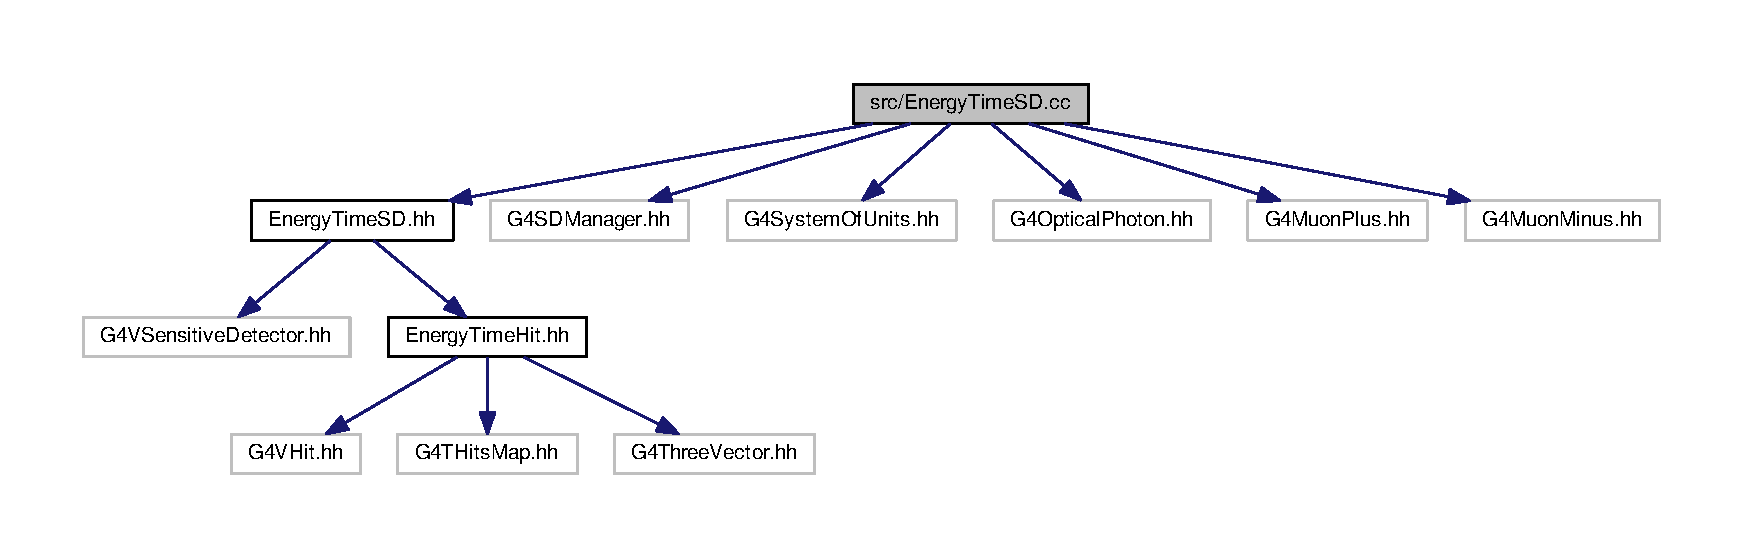
\includegraphics[width=350pt]{EnergyTimeSD_8cc__incl}
\end{center}
\end{figure}


\subsection{详细描述}
设置敏感探测器保存哪些数据 

muon 击中敏感探测器,保存时间,能量,位置和击中哪一个探测器信息 敏感探测器挂载在敏感探测器管理类格式为 name/energy\+\_\+time \begin{DoxyAuthor}{作者}
loyxin 
\end{DoxyAuthor}
\begin{DoxyVersion}{版本}
1.\+0 
\end{DoxyVersion}
\begin{DoxyDate}{日期}
2017-\/09-\/10 
\end{DoxyDate}
